% !TeX root = ../main.tex
% Copyright (c) 2026 Tyler Bignell
% Licensed under the MIT License - see LICENSE file for details

%%%%%%%%%%%%%%%%%%%%%%%%%%%%%%%%%%%%%%%%%%%%%%%%%%%%%%%%%%%
% FRONT MATTER
%%%%%%%%%%%%%%%%%%%%%%%%%%%%%%%%%%%%%%%%%%%%%%%%%%%%%%%%%%%
\begin{abstract} % Can use \metaAbstract from metadata or \input{} abstract optionally
This document is a beginner-friendly guide to this template. Each section introduces one or more packages included in the template, explains what it does in plain terms, and shows a simple working example. To get the most out of this file, open the compiled PDF and the source \texttt{example.tex} file side by side. Reading the code while looking at the result it produces is the fastest way to understand how each feature works.
\end{abstract}
\newpage

\tableofcontents
\newpage

\phantomsection % Allows TOC to link to todo list
\ifthenelse{\equal{\metaShowTodo}{true}}{%
	\addcontentsline{toc}{section}{Todo list}}{} % Creates TOC entry if metadata true
\listoftodos % Can be turned off in metadata

\phantomsection % Allows TOC to link to list of figures
\addcontentsline{toc}{section}{List of Figures} % Creates TOC entry
\listoffigures

\phantomsection % Allows TOC to link to list of tables
\addcontentsline{toc}{section}{List of Tables} % Creates TOC entry
\listoftables
\newpage

%%%%%%%%%%%%%%%%%%%%%%%%%%%%%%%%%%%%%%%%%%%%%%%%%%%%%%%%%%%
% CONDITIONALS
%%%%%%%%%%%%%%%%%%%%%%%%%%%%%%%%%%%%%%%%%%%%%%%%%%%%%%%%%%%
\section{Conditionals}

\subsection{\texttt{xifthen}}
\noindent\colorbox{themecolour!15}{\parbox{\linewidth}{\small This package is used internally by the template and is not typically invoked directly by the user.}}\vspace{0.5\baselineskip}

The \texttt{xifthen} package lets the template make simple yes/no decisions based on your metadata settings in \texttt{main.tex}. For example, it checks whether \texttt{\textbackslash metaShowTodo} is set to \texttt{true} and shows or hides the todo list accordingly. You do not need to write any \texttt{xifthen} commands yourself, just set your metadata values and the template handles the rest.

\subsection{\texttt{xstring}}
\noindent\colorbox{themecolour!15}{\parbox{\linewidth}{\small This package is used internally by the template for the smart header logic. Users do not use it directly.}}\vspace{0.5\baselineskip}

The \texttt{xstring} package gives the template tools to read and work with text strings. The template uses it to check the length of \texttt{\textbackslash metaCourseName} and decide whether to show the full name or a shorter acronym in the header. The table below shows what \texttt{xstring} can do:

\begin{table}[H]
	\centering
	\caption{Common \texttt{xstring} operations.}
	\label{tab:xstring}
	\begin{tabular}{@{}lll@{}}
		\toprule
		Operation & Command & Result \\
		\midrule
		Extraction   & \texttt{\textbackslash StrLeft\{Lassonde\}\{4\}}       & \StrLeft{Lassonde}{4} \\
		Substitution & \texttt{\textbackslash StrSubstitute\{12/05/26\}\{/\}\{-\}} & \StrSubstitute{12/05/26}{/}{-} \\
		Length       & \texttt{\textbackslash StrLen\{YorkU\}}                & \StrLen{YorkU} \\
		Counting     & \texttt{\textbackslash StrCount\{Engineering\}\{n\}}   & \StrCount{Engineering}{n} \\
		\bottomrule
	\end{tabular}
\end{table}

%%%%%%%%%%%%%%%%%%%%%%%%%%%%%%%%%%%%%%%%%%%%%%%%%%%%%%%%%%%
% COLOURS
%%%%%%%%%%%%%%%%%%%%%%%%%%%%%%%%%%%%%%%%%%%%%%%%%%%%%%%%%%%
\section{Colours}

\subsection{\texttt{xcolor}}
\noindent\colorbox{themecolour!15}{\parbox{\linewidth}{\small This package is used internally by the template for colour definitions and tints. Users may use it for custom colouring, but it is not required for normal document preparation.}}\vspace{0.5\baselineskip}

The \texttt{xcolor} package adds colour support to \LaTeX. The template uses it to apply your chosen theme colour to headings, horizontal rules, boxes, and highlighted notes throughout the document.

\subsubsection{Setting the Theme Colour}
You set the theme colour by editing \texttt{\textbackslash metaThemeColour} in \texttt{main.tex}. You can type a hex colour code, the name of any built-in colour, or the name of a custom colour defined in the template. If you leave it empty, the template uses \texttt{DefaultBlue}.

\begin{table}[H]
	\centering
	\caption{Accepted values for \texttt{\textbackslash metaThemeColour}.}
	\label{tab:theme-colour-values}
	\begin{tabularx}{\linewidth}{@{}llX@{}}
		\toprule
		Type & Example Value & Effect \\
		\midrule
		Empty         & \texttt{}        & Defaults to \texttt{DefaultBlue} \\
		Hex code      & \texttt{\#810001}  & Parsed as an HTML hex colour \\
		Named colour  & \texttt{red}     & Resolved via \texttt{\textbackslash colorlet} \\
		Custom colour & \texttt{LassondeNavy} & Any colour defined in the sty file \\
		\bottomrule
	\end{tabularx}
\end{table}

The same applies to \texttt{\textbackslash metaLinkColour}, \texttt{\textbackslash metaCiteColour}, and \texttt{\textbackslash metaUrlColour}; each one also falls back to \texttt{themecolour} when left empty.

\subsubsection{Custom Defined Colours}
These colours are built into the template and can be typed directly into \texttt{\textbackslash metaThemeColour} or any colour command:

\begin{table}[H]
	\centering
	\caption{Custom colours defined in \texttt{stemtemplate.sty}.}
	\label{tab:custom-colours}
	\begin{tabular}{@{}lll@{}}
		\toprule
		Name & Hex & Preview \\
		\midrule
		\texttt{DefaultBlue}  & \texttt{\#1B4F8A} & \textcolor{white}{\colorbox{DefaultBlue}{\phantom{XXXXX}}}  \\
		\texttt{YorkRedDark}     & \texttt{\#810001} & \textcolor{white}{\colorbox{YorkRedDark}{\phantom{XXXXX}}}     \\
		\texttt{ScienceSkyBlueDark}  & \texttt{\#065C87} & \textcolor{white}{\colorbox{ScienceSkyBlueDark}{\phantom{XXXXX}}}  \\
		\texttt{LassondeNavy} & \texttt{\#003366} & \textcolor{white}{\colorbox{LassondeNavy}{\phantom{XXXXX}}} \\
		\bottomrule
	\end{tabular}
\end{table}

\subsubsection{Built-in Named Colours}
You can also use any of \texttt{xcolor}'s built-in colour names. A small selection is shown below. For the full list, see \url{https://mirrors.ctan.org/macros/latex/contrib/xcolor/xcolor.pdf}:

\begin{table}[H]
	\centering
	\caption{Built-in \texttt{xcolor} named colours.}
	\label{tab:named-colours}
	\begin{tabular}{@{}llll@{}}
		\toprule
		Name & Preview & Name & Preview \\
		\midrule
		\multicolumn{4}{c}{\textit{Base colours}} \\
		\texttt{red}       	 & \colorbox{red}{\phantom{XXXXX}}       			& \texttt{cyan}      	 & \colorbox{cyan}{\phantom{XXXXX}}      \\
		\texttt{green}     	 & \colorbox{green}{\phantom{XXXXX}}     			& \texttt{magenta}     & \colorbox{magenta}{\phantom{XXXXX}}      \\
		\texttt{blue}   	 & \colorbox{blue}{\phantom{XXXXX}}   				& \texttt{yellow}    	 & \colorbox{yellow}{\phantom{XXXXX}}    \\
		\texttt{black}     	 & \colorbox{black}{\phantom{XXXXX}}     			& \texttt{white}     	 & \colorbox{white}{\phantom{XXXXX}}     \\
		\texttt{gray}  		 & \colorbox{gray}{\phantom{XXXXX}}  				& \texttt{brown}       & \colorbox{brown}{\phantom{XXXXX}}      \\
		\midrule
		\multicolumn{4}{c}{\textit{Extended colour sets (dvipsnames, svgnames, x11names})} \\
		\texttt{NavyBlue}    & \colorbox{NavyBlue}{\phantom{XXXXX}}      		& \texttt{ForestGreen} & \colorbox{ForestGreen}{\phantom{XXXXX}}     \\
		\texttt{Maroon}    	 & \colorbox{Maroon}{\phantom{XXXXX}}    			& \texttt{BurntOrange} & \colorbox{BurntOrange}{\phantom{XXXXX}}      \\
		\texttt{RoyalPurple} & \colorbox{RoyalPurple}{\phantom{XXXXX}}    		& \texttt{Sepia}       & \colorbox{Sepia}{\phantom{XXXXX}}      \\
		\texttt{SlateGray}   & \colorbox{SlateGray}{\phantom{XXXXX}}    		& \texttt{Teal}     	 & \colorbox{Teal}{\phantom{XXXXX}}     \\
		\texttt{SteelBlue4}	 & \colorbox{SteelBlue4}{\phantom{XXXXX}} 			& \texttt{Firebrick3}  & \colorbox{Firebrick3}{\phantom{XXXXX}}     \\
		\bottomrule
	\end{tabular}
\end{table}

\subsubsection{Theme Colour and Tints}
Adding \texttt{!} followed by a number after any colour name creates a lighter version of that colour, called a tint. The number is the percentage of the original colour --- so \texttt{themecolour!70} is 70\% colour and 30\% white. You can use any percentage directly inside any colour command:

\begin{table}[H]
	\centering
	\caption{Active theme colour and tints.}
	\label{tab:tints}
	\begin{tabular}{@{}lll@{}}
		\toprule
		Name & Tint & Preview \\
		\midrule
		\texttt{themecolour}     & 100\% & \textcolor{white}{\colorbox{themecolour}{\phantom{XXXXX}}} \\
		\texttt{themecolour!70}  & 70\%  & \textcolor{white}{\colorbox{themecolour!70}{\phantom{XXXXX}}} \\
		\texttt{themecolour!40}  & 40\%  & \colorbox{themecolour!40}{\phantom{XXXXX}} \\
		\texttt{themecolour!15}  & 15\%  & \colorbox{themecolour!15}{\phantom{XXXXX}} \\
		\bottomrule
	\end{tabular}
\end{table}

\subsubsection{Using \texttt{\textbackslash textcolor} and \texttt{\textbackslash colorbox}}
Use \texttt{\textbackslash textcolor} to change the colour of a word or phrase in your text. It takes two arguments: the colour name and the text to colour. For example, \textcolor{themecolour}{\texttt{\textbackslash textcolor\{themecolour\}\{Sample Text\}}} colours the text without changing anything else on the line.

Use \texttt{\textbackslash colorbox} to place a coloured background behind text, useful for drawing attention to a short note or label. For example, \colorbox{themecolour!15}{\texttt{\textbackslash colorbox\{themecolour!15\}\{Sample Text\}}} produces a lightly shaded highlight box.

%%%%%%%%%%%%%%%%%%%%%%%%%%%%%%%%%%%%%%%%%%%%%%%%%%%%%%%%%%%
% PAGE GEOMETRY
%%%%%%%%%%%%%%%%%%%%%%%%%%%%%%%%%%%%%%%%%%%%%%%%%%%%%%%%%%%
\section{Page Geometry}

\subsection{\texttt{geometry}}
\noindent\colorbox{themecolour!15}{\parbox{\linewidth}{\small This package is used internally by the template to configure page margins and layout. Users do not normally modify these settings.}}\vspace{0.5\baselineskip}

The \texttt{geometry} package controls the page margins and the size of the text area. The template uses it to set standard margins automatically, you do not need to touch anything for your document to be formatted correctly.

\subsection{\texttt{setspace}}
\noindent\colorbox{themecolour!15}{\parbox{\linewidth}{\small This package is used internally by the template to control line spacing. Users normally do not interact with it directly, but spacing can be adjusted through metadata commands in \texttt{main.tex}.}}\vspace{0.5\baselineskip}

The \texttt{setspace} package controls the space between lines of text. You can choose between single, one-and-a-half, or double spacing by setting the appropriate metadata value in \texttt{main.tex}, you do not need to call any \texttt{setspace} commands yourself.

\begin{landscape} 	  % Begins landscape
\thispagestyle{plain} % Removes header from landscape page
\subsection{\texttt{pdflscape}}
\noindent\colorbox{themecolour!15}{\parbox{\linewidth}{\small This package is available for rotating wide tables or figures into landscape orientation. It is not required for normal document preparation and is only used when the author explicitly includes a landscape environment.}}\vspace{0.5\baselineskip}

The \texttt{pdflscape} package lets you rotate a page sideways so that wide content fits. Wrap anything in a \texttt{landscape} environment and that page will display in landscape orientation in the PDF viewer. The page after it returns to portrait automatically.

The table below is an example of content that is too wide for portrait and benefits from a landscape page:

\begin{table}[H]
	\centering
	\caption{Wide data table spanning landscape page.}
	\label{tab:landscape}
	\begin{tabularx}{\linewidth}{@{}lXXXXX@{}}
		\toprule
		Parameter & Trial 1 & Trial 2 & Trial 3 & Trial 4 & Trial 5 \\
		\midrule
		Temperature (\si{\celsius})     & 23.4 & 24.1 & 22.8 & 23.9 & 24.5 \\
		Pressure (\si{\kilo\pascal})  & 101.3 & 101.1 & 101.5 & 100.9 & 101.4 \\
		Humidity (\%)               & 48.7 & 50.2 & 47.9 & 51.0 & 49.3 \\
		Voltage (\si{\volt})          & 4.98 & 5.01 & 4.97 & 5.02 & 5.00 \\
		Current (\si{\milli\ampere}) & 120.1 & 119.8 & 120.4 & 120.0 & 119.6 \\
		\bottomrule
	\end{tabularx}
\end{table}

Use \texttt{$\backslash$thispagestyle\{plain\}} on the line after \texttt{$\backslash$begin\{landscape\}} to remove the header from the rotated page. Use \texttt{$\backslash$thispagestyle\{empty\}} instead if you also want to hide the page number in the footer.
\end{landscape} % Ends landscape

%%%%%%%%%%%%%%%%%%%%%%%%%%%%%%%%%%%%%%%%%%%%%%%%%%%%%%%%%%%
% LANGUAGE
%%%%%%%%%%%%%%%%%%%%%%%%%%%%%%%%%%%%%%%%%%%%%%%%%%%%%%%%%%%
\section{Language}

\subsection{\texttt{inputenc}}
\noindent\colorbox{themecolour!15}{\parbox{\linewidth}{\small This package ensures that UTF-8 characters are interpreted correctly. It is loaded automatically by the template and normally does not require user modification.}}\vspace{0.5\baselineskip}

The \texttt{inputenc} package lets you type accented and special characters such as \texttt{é}, \texttt{ö}, \texttt{ñ}, and \texttt{ç} directly in your source file without any extra commands. The template loads it automatically so you never need to think about it.

\subsection{\texttt{fontenc}}
\noindent\colorbox{themecolour!15}{\parbox{\linewidth}{\small This package controls the output font encoding used when generating the PDF. It is loaded automatically by the template and normally does not require user modification.}}\vspace{0.5\baselineskip}

The \texttt{fontenc} package controls how characters are stored in the PDF. The template uses the \texttt{T1} encoding so that accented characters display correctly, words hyphenate properly, and text can be copied out of the PDF cleanly. It is applied automatically with no action needed from you.

\subsection{\texttt{babel}}
\noindent\colorbox{themecolour!15}{\parbox{\linewidth}{\small This package manages language-specific typographic rules. The template loads it automatically with English as the active language.}}\vspace{0.5\baselineskip}

The \texttt{babel} package tells \LaTeX{} which language the document is written in. The template loads it with English so that words are hyphenated correctly and punctuation follows English conventions. No changes are needed on your end.

%%%%%%%%%%%%%%%%%%%%%%%%%%%%%%%%%%%%%%%%%%%%%%%%%%%%%%%%%%%
% FONT SELECTION
%%%%%%%%%%%%%%%%%%%%%%%%%%%%%%%%%%%%%%%%%%%%%%%%%%%%%%%%%%%
\section{Font Selection}

\subsection{\texttt{plex-serif} and \texttt{\textbackslash seriftext}}
\noindent\colorbox{themecolour!15}{\parbox{\linewidth}{\small Loaded automatically to control the serif font. Users typically only use the \texttt{\textbackslash seriftext\{\}} command, not the package itself.}}\vspace{0.5\baselineskip}

The \texttt{plex-serif} package loads IBM Plex Serif, a readable serif font. You can apply it to any word or phrase using \texttt{\textbackslash seriftext\{\}}:

\seriftext{This text is rendered in IBM Plex Serif (serif font).}

This is handy when your document is set to sans-serif by default but you want a specific word or phrase to appear in serif instead.

\subsection{\texttt{plex-sans} and \texttt{\textbackslash sansseriftext}}
\noindent\colorbox{themecolour!15}{\parbox{\linewidth}{\small Loaded automatically to control the sans-serif font. Users normally interact with it only through \texttt{\textbackslash sansseriftext\{\}}.}}\vspace{0.5\baselineskip}

The \texttt{plex-sans} package loads IBM Plex Sans, a readable sans-serif font. You can apply it to any word or phrase using \texttt{\textbackslash sansseriftext\{\}}:

\sansseriftext{This text is rendered in IBM Plex Sans (sans-serif font).}

This is handy when your document is set to serif by default but you want a specific word or phrase to appear in sans-serif instead.

\subsection{Default Font}
\noindent\colorbox{themecolour!15}{\parbox{\linewidth}{\small The template selects the global font through the metadata in \texttt{main.tex}; users typically do not modify font packages directly.}}\vspace{0.5\baselineskip}

You control the font for the whole document by setting \texttt{\textbackslash metaDefaultFont} in \texttt{main.tex}. The current setting is \texttt{\metaDefaultFont}. Set it to \texttt{serif} for IBM Plex Serif or \texttt{sans} for IBM Plex Sans. The local commands \texttt{\textbackslash seriftext\{\}} and \texttt{\textbackslash sansseriftext\{\}} still work regardless of which global font you choose.

%%%%%%%%%%%%%%%%%%%%%%%%%%%%%%%%%%%%%%%%%%%%%%%%%%%%%%%%%%%
% SPACING AROUND HEADINGS
%%%%%%%%%%%%%%%%%%%%%%%%%%%%%%%%%%%%%%%%%%%%%%%%%%%%%%%%%%%
\section{Spacing Around Headings}

\subsection{\texttt{titlesec}}
\noindent\colorbox{themecolour!15}{\parbox{\linewidth}{\small This package is used by the template to control heading formatting and spacing. Users typically do not modify it directly.}}\vspace{0.5\baselineskip}

The \texttt{titlesec} package controls how headings look throughout the document. The template uses it to make all headings bold and coloured with \texttt{themecolour}. You do not need to change anything here.

\subsubsection{Abstract environment}
\noindent\colorbox{themecolour!15}{\parbox{\linewidth}{\small The abstract environment is customised by the template to ensure consistent formatting. Users typically write their abstract normally without modifying this configuration.}}\vspace{0.5\baselineskip}

By default, \LaTeX{} centres the abstract text in italic. The template overrides this so the abstract looks like a regular section heading instead, which is the bold flush-left ``Abstract'' heading you see at the start of this document. You write your abstract the same way either way, just inside \texttt{\textbackslash begin\{abstract\}} and \texttt{\textbackslash end\{abstract\}}.

The title page uses a separate version of the abstract that keeps the original centred style, so both layouts are available depending on where the abstract appears.

%%%%%%%%%%%%%%%%%%%%%%%%%%%%%%%%%%%%%%%%%%%%%%%%%%%%%%%%%%%
% MATH
%%%%%%%%%%%%%%%%%%%%%%%%%%%%%%%%%%%%%%%%%%%%%%%%%%%%%%%%%%%
\section{Math}

\subsection{\texttt{amsmath}, \texttt{amssymb}, \texttt{amsfonts}}
These three packages are the standard tools for writing math in \LaTeX. Together they give you display math environments, a large collection of math symbols, and blackboard bold letters for number sets like $\mathbb{R}$, $\mathbb{Z}$, and $\mathbb{N}$.

The \texttt{equation} environment puts a single equation on its own line with a number on the right. Use \texttt{equation*} if you do not want the number:

\begin{equation}
	2 + 2 = 4
	\label{eq:simple}
\end{equation}

\begin{equation}
	\boxed{a^2 + b^2 = c^2}
	\label{eq:pythagoras}
\end{equation}

The \texttt{align} environment lets you write multiple equations that line up at the \texttt{\&} character. Each line gets its own number unless you add \texttt{\textbackslash nonumber} to that line:

\begin{align}
	y &= 2x + 1 \\
	&= 2(3) + 1 \nonumber
\end{align}

The \texttt{gather} environment puts each equation on its own centred line with no alignment between them. Use it when you have a group of separate equations to display together:

\begin{gather}
	x + y = 5 \\
	x - y = 1
\end{gather}

The \texttt{split} environment breaks one long equation across multiple lines while keeping a single equation number. It must be placed inside \texttt{equation}:

\begin{equation}
	\begin{split}
		(a + b)^2 &= a^2 + 2ab \\
		&\quad + b^2
	\end{split}
\end{equation}

The \texttt{cases} environment is used for piecewise functions. It draws an opening brace and lets you write a different expression for each condition:

\begin{equation}
	|x| = \begin{cases}
		x  & \text{if } x \geq 0 \\
		-x & \text{if } x < 0
	\end{cases}
\end{equation}

The \texttt{multline} environment is for a single equation that is too long to fit on one line. The first line is left-aligned, the last line is right-aligned, and any lines in between are centred:

\begin{multline}
	(a_1 + a_2 + a_3) \times (b_1 + b_2 + b_3) = \\
	a_1 b_1 + a_1 b_2 + a_1 b_3 + a_2 b_1 + a_2 b_2 + \\
	a_2 b_3 + a_3 b_1 + a_3 b_2 + a_3 b_3
\end{multline}

\subsection{\texttt{mathtools}}
The \texttt{mathtools} package adds a few extra tools on top of \texttt{amsmath}. The most useful for everyday writing is \texttt{\textbackslash coloneqq}, which produces the ``defined as equal to'' symbol:

\begin{equation}
	f(x) \coloneqq 2x + 3
\end{equation}

It also provides matrix environments with different bracket styles. Each one works the same way but uses different surrounding symbols:

\begin{equation}
	\text{pmatrix: }
	\begin{pmatrix} a & b \\ c & d \end{pmatrix} \qquad
	\text{bmatrix: }
	\begin{bmatrix} a & b \\ c & d \end{bmatrix} \qquad
	\text{vmatrix: }
	\begin{vmatrix} a & b \\ c & d \end{vmatrix} \qquad
	\text{Vmatrix: }
	\begin{Vmatrix} a & b \\ c & d \end{Vmatrix}
\end{equation}

\subsection{\texttt{bm}}
The \texttt{bm} package gives you the \texttt{\textbackslash bm\{\}} command, which makes a math symbol bold while keeping it italic. This is the standard way to write vectors and matrices in science and engineering, since \texttt{\textbackslash mathbf} would make the letter upright:

\begin{equation}
	\bm{F} = m\bm{a} \qquad \bm{v} = \bm{u} + \bm{a}t
\end{equation}

\subsection{\texttt{siunitx}}
The \texttt{siunitx} package formats numbers and units correctly. Use \texttt{\textbackslash SI\{value\}\{unit\}} when you have a number and a unit together, and \texttt{\textbackslash si\{unit\}} when you just need the unit on its own.

\begin{table}[H]
	\centering
	\label{tab:siunitx}
	\caption{SI unit examples using \texttt{siunitx}.}
	\begin{tabularx}{\linewidth}{@{}lX@{}}
		\toprule
		Command & Output \\
		\midrule
		\texttt{\textbackslash SI\{9.81\}\{\textbackslash metre\textbackslash per\textbackslash second\textbackslash squared\}} & \SI{9.81}{\metre\per\second\squared} \\
		\texttt{\textbackslash SI\{3e8\}\{\textbackslash metre\textbackslash per\textbackslash second\}} & \SI{3e8}{\metre\per\second} \\
		\texttt{\textbackslash SI\{100\}\{\textbackslash kilo\textbackslash gram\}} & \SI{100}{\kilo\gram} \\
		\texttt{\textbackslash SI\{1.6e-19\}\{\textbackslash coulomb\}} & \SI{1.6e-19}{\coulomb} \\
		\texttt{\textbackslash si\{\textbackslash ohm\}} & \si{\ohm} \\
		\texttt{\textbackslash si\{\textbackslash kilo\textbackslash pascal\}} & \si{\kilo\pascal} \\
		\bottomrule
	\end{tabularx}
\end{table}

Units can also be used inline inside a sentence. For example, gravitational acceleration is \SI{9.81}{\metre\per\second\squared}, and standard atmospheric pressure is \SI{101.325}{\kilo\pascal}.

\subsection{\texttt{mhchem}}
The \texttt{mhchem} package lets you write chemical formulas and reactions using the \texttt{\textbackslash ce\{\}} command. You just type the formula naturally and it handles all the subscripts, superscripts, and charges for you.

You can use it inline inside a sentence: water is \ce{H2O}, table salt is \ce{NaCl}, and the sulfate ion is \ce{SO4^2-}.

To show a reaction on its own line, place \texttt{\textbackslash ce} inside an \texttt{equation} environment:

\begin{equation}
	\ce{2H2 + O2 -> 2H2O}
\end{equation}

\begin{equation}
	\ce{A + B <=> C + D}
\end{equation}

Adding \texttt{->[\textbackslash Delta][Heat]} puts a delta above the arrow, and text below it which is commonly used to show that heat or a catalyst is applied:

\begin{equation}
	\ce{A ->[\Delta] B}
\end{equation}

\begin{equation}
	\ce{A ->[\Delta][Heat] B}
\end{equation}

You can also write isotopes by putting the mass number and atomic number before the element symbol:

\begin{equation}
	\ce{^{235}_{92}U + ^{1}_{0}n -> ^{141}_{56}Ba + ^{92}_{36}Kr + 3^{1}_{0}n}
\end{equation}

%%%%%%%%%%%%%%%%%%%%%%%%%%%%%%%%%%%%%%%%%%%%%%%%%%%%%%%%%%%
% THEOREM ENVIRONMENTS
%%%%%%%%%%%%%%%%%%%%%%%%%%%%%%%%%%%%%%%%%%%%%%%%%%%%%%%%%%%
\section{Theorem Environments}

\subsection{\texttt{amsthm}}
The \texttt{amsthm} package gives you styled boxes for presenting formal mathematical statements. The template defines three visual styles: \texttt{plain}, \texttt{definition}, and \texttt{remark}. Each style is used by a different group of environments shown below.

\subsubsection{Plain --- Theorem, Lemma, Proposition, Corollary, Conjecture, Axiom, Proof}

\begin{theorem}
	\label{thm:pythagorean}
	For any right triangle with sides $a$ and $b$ and hypotenuse $c$:
	$a^2 + b^2 = c^2$.
\end{theorem}

\begin{proof}
	Draw a square on each side of the triangle and compare the areas.
\end{proof}

The end-of-proof symbol \texttt{\textbackslash qed} is redefined in \texttt{stemtemplate.sty} to show a solid \texttt{themecolour} square (\textcolor{themecolour}{$\blacksquare$}) instead of the default hollow box.

\begin{lemma}
	\label{lem:even}
	If $n$ is an even number, then $n^2$ is also even.
\end{lemma}

\begin{proposition}
	\label{prop:rational}
	The sum of two whole-number fractions is always a whole-number fraction.
\end{proposition}

\begin{corollary}
	\label{cor:prime}
	If $p$ is a prime number greater than 2, then $p$ is odd.
\end{corollary}

\begin{conjecture}
	\label{con:goldbach}
	Every even number greater than 2 can be written as the sum of two prime numbers.
\end{conjecture}

\begin{axiom}
	\label{axm:line}
	Through any two points there is exactly one straight line.
\end{axiom}

\subsubsection{Definition --- Definition, Example, Criterion}

\begin{definition}
	\label{def:even}
	An even number is any integer that can be divided by 2 with no remainder.
\end{definition}

\begin{example}
	\label{ex:even}
	The numbers 2, 4, 6, and 8 are all even numbers.
\end{example}

\begin{criterion}
	\label{crit:positive}
	A number is positive if and only if it is greater than zero.
\end{criterion}

\subsubsection{Remark --- Remark, Note}

\begin{remark}
	\label{rem:zero}
	Zero is even because it can be divided by 2 with no remainder.
\end{remark}

\begin{note}
	\label{note:numbering}
	All theorem environments are automatically numbered by section when \texttt{\textbackslash metaNumberTheorems} is set to \texttt{true}.
\end{note}

%%%%%%%%%%%%%%%%%%%%%%%%%%%%%%%%%%%%%%%%%%%%%%%%%%%%%%%%%%%
% GRAPHICS, FIGURES & TABLES
%%%%%%%%%%%%%%%%%%%%%%%%%%%%%%%%%%%%%%%%%%%%%%%%%%%%%%%%%%%
\section{Graphics, Figures \& Tables}

\subsection{\texttt{graphicx}}
The \texttt{graphicx} package provides the \texttt{\textbackslash includegraphics} command for placing images in your document. The template is set up to look for images in the \texttt{figures/} and \texttt{assets/} folders, so you only need to type the filename with no folder path.

You can control the size of the image with optional arguments: \texttt{width=0.6\textbackslash linewidth} scales it to 60\% of the text width, \texttt{height=5cm} sets a fixed height, and \texttt{scale=0.5} makes it half its original size. You only need to set one of these and the other dimension scales automatically to keep the proportions correct.

\begin{figure}[H]
	\centering
	\includegraphics[width=0.6\linewidth]{\metaLogoPath}
	\caption{Faculty logo included with \texttt{\textbackslash includegraphics}.}
	\label{fig:logo}
\end{figure}

\subsection{\texttt{booktabs}}
The \texttt{booktabs} package gives you three horizontal line commands for clean, professional tables: \texttt{\textbackslash toprule} at the top, \texttt{\textbackslash midrule} between the header row and the data, and \texttt{\textbackslash bottomrule} at the bottom. Always use these instead of \texttt{\textbackslash hline}.

\begin{table}[H]
	\centering
	\caption{Basic table using \texttt{booktabs}.}
	\label{tab:booktabs}
	\begin{tabular}{@{}lcc@{}}
		\toprule
		Parameter & Value & Unit \\
		\midrule
		Resistance & 10 & \si{\ohm} \\
		Current    & 2  & \si{\ampere} \\
		Voltage    & 20 & \si{\volt} \\
		\bottomrule
	\end{tabular}
\end{table}

\subsection{\texttt{array}}
\noindent\colorbox{themecolour!15}{\parbox{\linewidth}{\small This package is used internally by the template and is required by \texttt{tabularx} and \texttt{multirow}. Users may use its column specifiers directly when fine-grained column control is needed.}}\vspace{0.5\baselineskip}

The \texttt{array} package lets you apply formatting to an entire column at once. The \texttt{>{\ldots}} syntax goes before the column letter in your column definition and applies a command to every cell in that column. The example below uses it to centre and wrap text in two fixed-width columns:

\begin{table}[H]
	\centering
	\caption{Fixed-width centred columns using \texttt{array}.}
	\label{tab:array}
	\begin{tabular}{>{\centering\arraybackslash}p{4cm} >{\centering\arraybackslash}p{4cm}}
		\toprule
		Left column & Right column \\
		\midrule
		Centred text & Centred text \\
		Long cell content wraps & Also wraps cleanly \\
		\bottomrule
	\end{tabular}
\end{table}

\subsection{\texttt{tabularx}}
The \texttt{tabularx} package adds the \texttt{X} column type, which automatically stretches to fill the remaining width of the table. You set the total table width as the first argument (usually \texttt{\textbackslash linewidth}) and any \texttt{X} columns share the leftover space equally. This is the preferred table environment in this template.

\begin{table}[H]
	\centering
	\caption{Auto-width table using \texttt{tabularx}.}
	\label{tab:tabularx}
	\begin{tabularx}{\linewidth}{@{}lccX@{}}
		\toprule
		Parameter & Value & Unit & Description \\
		\midrule
		Resistance & 10 & \si{\ohm} & Opposition to current flow in a circuit \\
		Current    & 2  & \si{\ampere} & Flow of electric charge through a conductor \\
		Voltage    & 20 & \si{\volt} & Electric potential difference between two points \\
		\bottomrule
	\end{tabularx}
\end{table}

\subsection{\texttt{multirow}}
The \texttt{multirow} package lets a single cell span more than one row. The command is \texttt{\textbackslash multirow\{n\}\{width\}\{content\}}, where \texttt{n} is the number of rows to span and \texttt{width} is usually \texttt{*} to let \LaTeX{} set it automatically. Leave the cells below the merged cell empty. Adding a \texttt{\textbackslash midrule} between groups helps separate them visually:

\begin{table}[H]
	\centering
	\caption{Table with multi-row cells using \texttt{multirow}.}
	\label{tab:multirow}
	\begin{tabular}{@{}llc@{}}
		\toprule
		Category & Parameter & Value \\
		\midrule
		\multirow{2}{*}{Electrical} & Resistance & \SI{10}{\ohm} \\
		& Current    & \SI{2}{\ampere} \\
		\midrule
		\multirow{2}{*}{Mechanical} & Force    & \SI{50}{\newton} \\
		& Velocity & \SI{3}{\metre\per\second} \\
		\bottomrule
	\end{tabular}
\end{table}

\subsection{\texttt{longtable}}
The \texttt{longtable} environment is used when a table is too long to fit on one page. It handles page breaks automatically and repeats the header row at the top of each new page. Define the header once inside \texttt{\textbackslash endfirsthead} for the first page and again inside \texttt{\textbackslash endhead} for all following pages. The closing rule goes inside \texttt{\textbackslash endfoot}:

\begin{longtable}{@{}lcc@{}}
	\caption{A long table that spans multiple pages.}
	\label{tab:longtable} \\
	\toprule
	Parameter & Value & Unit \\
	\midrule
	\endfirsthead
	\toprule
	Parameter & Value & Unit \\
	\midrule
	\endhead
	\bottomrule
	\endfoot
	Row 1  & 1  & \si{\ohm} \\
	Row 2  & 2  & \si{\ohm} \\
	Row 3  & 3  & \si{\ohm} \\
	Row 4  & 4  & \si{\ohm} \\
	Row 5  & 5  & \si{\ohm} \\
	Row 6  & 6  & \si{\ohm} \\
	Row 7  & 7  & \si{\ohm} \\
	Row 8  & 8  & \si{\ohm} \\
	Row 9  & 9  & \si{\ohm} \\
	Row 10 & 10 & \si{\ohm} \\
\end{longtable}

\subsection{\texttt{float}}
This package is used internally by the template to enable the \texttt{[H]} placement specifier. Users interact with it by adding \texttt{[H]} to any \texttt{figure} or \texttt{table} environment.

\subsection{\texttt{subcaption}}
The \texttt{subcaption} package lets you place two or more related figures or tables side by side under a shared caption. Each one gets its own label and caption, and the group gets a shared parent label. They are lettered automatically as (a), (b), (c), and so on.

\begin{figure}[H]
	\centering
	\begin{subfigure}[b]{0.45\linewidth}
		\centering
		\includegraphics[width=\linewidth]{\metaLogoPath}
		\caption{First sub-figure.}
		\label{fig:sub_a}
	\end{subfigure}
	\hfill
	\begin{subfigure}[b]{0.45\linewidth}
		\centering
		\includegraphics[width=\linewidth]{\metaLogoPath}
		\caption{Second sub-figure.}
		\label{fig:sub_b}
	\end{subfigure}
	\caption{Two sub-figures using \texttt{subcaption}.}
	\label{fig:subfigs}
\end{figure}

\subsection{\texttt{caption}}
\noindent\colorbox{themecolour!15}{\parbox{\linewidth}{\small This package is used internally by the template to define caption formatting. Users do not modify it directly; captions are written normally with \texttt{\textbackslash caption\{\}}.}}\vspace{0.5\baselineskip}

The \texttt{caption} package controls how figure and table captions look. The template uses it to make the label bold and coloured in \texttt{themecolour}, followed by a colon, with the caption text left-aligned in a slightly smaller font. This applies automatically to every \texttt{\textbackslash caption} in your document with no extra work needed.

\subsection{\texttt{pdfpages}}
The \texttt{pdfpages} package lets you insert pages from another PDF directly into your document using \texttt{\textbackslash includepdf[options]\{filename.pdf\}}. By default the inserted pages have no header or footer. Pass \texttt{pagecommand=\{\textbackslash thispagestyle\{fancy\}\}} to bring them back.

\begin{table}[H]
	\centering
	\caption{Common \texttt{\textbackslash includepdf} options.}
	\label{tab:pdfpages}
	\begin{tabularx}{\linewidth}{@{}lX@{}}
		\toprule
		Option & Effect \\
		\midrule
		\texttt{pages=-}        & Include all pages \\
		\texttt{pages=\{1,3\}}  & Include pages 1 and 3 only \\
		\texttt{pages=\{2-5\}}  & Include a page range \\
		\texttt{landscape}      & Rotate inserted pages to landscape \\
		\texttt{nup=2x1}        & Place two source pages side by side on one sheet \\
		\texttt{pagecommand=\{\textbackslash thispagestyle\{fancy\}\}} & Restore header and footer on inserted pages \\
		\bottomrule
	\end{tabularx}
\end{table}

%%%%%%%%%%%%%%%%%%%%%%%%%%%%%%%%%%%%%%%%%%%%%%%%%%%%%%%%%%%
% DIAGRAMS & PLOTS
%%%%%%%%%%%%%%%%%%%%%%%%%%%%%%%%%%%%%%%%%%%%%%%%%%%%%%%%%%%
\section{Diagrams \& Plots}

\subsection{\texttt{tikz}}
The \texttt{tikz} package lets you draw diagrams directly in your document using simple drawing commands. Everything is described with coordinates and paths in code, so diagrams scale perfectly and can include \LaTeX{} math and text naturally.

The basic drawing command is \texttt{\textbackslash draw[options] (start) -- (end);}. The \texttt{->} option adds an arrowhead and \texttt{rectangle} draws a box between two corner coordinates. Coordinates are written as \texttt{(x,y)} in centimetres by default.

\begin{figure}[H]
	\centering
	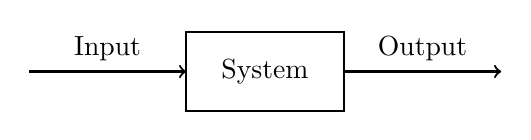
\begin{tikzpicture}
		\draw[thick, ->, color=black] (0,0) -- (2,0) node[midway, above] {Input};
		\draw[thick, color=black] (2,-0.5) rectangle (4,0.5) node[midway] {System};
		\draw[thick, ->, color=black] (4,0) -- (6,0) node[midway, above] {Output};
	\end{tikzpicture}
	\caption{Simple block diagram drawn with \texttt{tikz}.}
	\label{fig:tikz}
\end{figure}

\subsection{\texttt{pgfplots}}
The \texttt{pgfplots} package builds data plots on top of \texttt{tikz}. Plots go inside an \texttt{axis} environment, which handles the axis labels, tick marks, grid lines, and scaling for you. Use \texttt{\textbackslash addplot\{expression\}} to plot a mathematical function, or supply explicit coordinates to plot data points.

Useful axis options include \texttt{width}, \texttt{height}, \texttt{xlabel}, \texttt{ylabel}, \texttt{xmin}/\texttt{xmax}, \texttt{ymin}/\texttt{ymax}, and \texttt{grid}. The \texttt{domain} option on \texttt{\textbackslash addplot} sets the range of $x$ values and \texttt{samples} controls how smooth the curve looks.

\begin{figure}[H]
	\centering
	\begin{tikzpicture}
		\begin{axis}[
			width=0.75\linewidth,
			height=5cm,
			xlabel={$x$},
			ylabel={$y$},
			grid=major,
			grid style={color=themecolour!20},
			title={\textrm{Title (Exclude this, figure caption acts as a title)}},
			legend style={at={(1.02,0.5)}, anchor=west}]
			\addplot[color=themecolour, thick, domain=0:360, samples=100] {sin(x)};
			\addlegendentry{$\sin(x)$}
			\addplot[color=themecolour!40, thick, domain=0:360, samples=100] {cos(x)};
			\addlegendentry{$\cos(x)$}
		\end{axis}
	\end{tikzpicture}
	\caption{Sine and cosine waves plotted with \texttt{pgfplots}.}
	\label{fig:pgfplots}
\end{figure}

\subsection{\texttt{circuitikz}}
The \texttt{circuitikz} package extends \texttt{tikz} with circuit symbols for drawing electrical schematics. Components are placed along a path using \texttt{to[component, label]}, where the component name is a standard symbol such as \texttt{R} (resistor), \texttt{C} (capacitor), \texttt{L} (inductor), \texttt{V} (voltage source), or \texttt{I} (current source). Paths are chained together to form a closed loop.

\begin{figure}[H]
	\centering
	\begin{circuitikz}
		\draw (0,0)
		to[V, l=$V_s$] (0,2)
		to[R, l=$R$]   (2,2)
		to[C, l=$C$]   (2,0)
		-- (0,0);
	\end{circuitikz}
	\caption{Simple RC circuit drawn with \texttt{circuitikz}.}
	\label{fig:circuit}
\end{figure}

%%%%%%%%%%%%%%%%%%%%%%%%%%%%%%%%%%%%%%%%%%%%%%%%%%%%%%%%%%%
% ALGORITHMS
%%%%%%%%%%%%%%%%%%%%%%%%%%%%%%%%%%%%%%%%%%%%%%%%%%%%%%%%%%%
\section{Algorithms}

\subsection{\texttt{algorithm} and \texttt{algpseudocode}}
The \texttt{algorithm} package provides a float wrapper for pseudocode, giving algorithms captions, labels, and an entry in a list of algorithms, the same way \texttt{figure} wraps a \texttt{tikzpicture}. The \texttt{algpseudocode} package supplies the pseudocode commands that go inside the \texttt{algorithmic} environment.

The \texttt{algorithmic} environment takes an optional line-numbering argument: \texttt{[1]} numbers every line, \texttt{[2]} numbers every second line, and omitting it disables numbering entirely.

\begin{table}[H]
	\centering
	\caption{Common \texttt{algpseudocode} commands.}
	\label{tab:algpseudocode}
	\begin{tabularx}{\linewidth}{@{}lX@{}}
		\toprule
		Command & Purpose \\
		\midrule
		\texttt{\textbackslash Require} & Declares what the algorithm expects as input \\
		\texttt{\textbackslash Ensure}  & Declares what the algorithm produces as output \\
		\texttt{\textbackslash State}   & A single statement on its own line \\
		\texttt{\textbackslash Function\{name\}\{params\}} & Opens a named function block \\
		\texttt{\textbackslash If / \textbackslash ElsIf / \textbackslash Else / \textbackslash EndIf} & Conditional branch \\
		\texttt{\textbackslash For / \textbackslash EndFor} & For loop \\
		\texttt{\textbackslash While / \textbackslash EndWhile} & While loop \\
		\texttt{\textbackslash Return} & Return statement \\
		\texttt{\textbackslash Comment\{...\}} & Inline comment, right-aligned \\
		\bottomrule
	\end{tabularx}
\end{table}

The two algorithms below demonstrate a function with nested control flow. Indentation is handled automatically with no manual spacing required:

\begin{algorithm}[H]
	\caption{Binary Search}
	\label{alg:binarysearch}
	\begin{algorithmic}[1]
		\Require Sorted array $A$ of length $n$, search value $target$
		\Ensure Index of $target$ in $A$, or $-1$ if not found
		\Function{BinarySearch}{$A, n, target$}
		\State $low \gets 0$
		\State $high \gets n - 1$
		\While{$low \leq high$}
		\State $mid \gets \lfloor(low + high) / 2\rfloor$ \Comment{Compute midpoint}
		\If{$A[mid] = target$}
		\State \Return $mid$ \Comment{Target found}
		\ElsIf{$A[mid] < target$}
		\State $low \gets mid + 1$ \Comment{Search right half}
		\Else
		\State $high \gets mid - 1$ \Comment{Search left half}
		\EndIf
		\EndWhile
		\State \Return $-1$ \Comment{Target not found}
		\EndFunction
	\end{algorithmic}
\end{algorithm}

\begin{algorithm}[H]
	\caption{Bubble Sort}
	\label{alg:bubblesort}
	\begin{algorithmic}[1]
		\Require Array $A$ of length $n$
		\Ensure $A$ sorted in ascending order
		\Function{BubbleSort}{$A, n$}
		\For{$i \gets 0$ \textbf{to} $n - 1$}
		\For{$j \gets 0$ \textbf{to} $n - i - 2$}
		\If{$A[j] > A[j+1]$}
		\State swap $A[j]$ and $A[j+1]$ \Comment{Swap out-of-order elements}
		\EndIf
		\EndFor
		\EndFor
		\EndFunction
	\end{algorithmic}
\end{algorithm}

Algorithms are referenced using \texttt{\textbackslash cref} like any other float. \cref{alg:binarysearch} searches a sorted list by repeatedly halving the search range, while \cref{alg:bubblesort} sorts a list by repeatedly swapping neighbouring elements that are in the wrong order.

%%%%%%%%%%%%%%%%%%%%%%%%%%%%%%%%%%%%%%%%%%%%%%%%%%%%%%%%%%%
% LINKS & REFERENCES
%%%%%%%%%%%%%%%%%%%%%%%%%%%%%%%%%%%%%%%%%%%%%%%%%%%%%%%%%%%
\section{Links \& References}

\subsection{\texttt{hyperref}}
\noindent\colorbox{themecolour!15}{\parbox{\linewidth}{\small This package is used internally by the template to configure clickable links and PDF metadata. Users interact with it through \texttt{\textbackslash url\{\}} and \texttt{\textbackslash href\{\}\{\}} for external links; all internal cross-references are handled automatically.}}\vspace{0.5\baselineskip}

The \texttt{hyperref} package makes every internal cross-reference, citation, and table of contents entry clickable in the PDF. It also embeds document information such as the title and author into the PDF file. The template sets all link colours to \texttt{themecolour} automatically.

The two commands you will use directly are \texttt{\textbackslash url\{\}} for a plain clickable link and \texttt{\textbackslash href\{url\}\{text\}} for a link with custom display text:

\begin{itemize}[noitemsep]
	\item \texttt{\textbackslash url\{https://www.yorku.ca\}} $\to$ \url{https://www.yorku.ca}
	\item \texttt{\textbackslash href\{https://www.yorku.ca\}\{York University\}} $\to$ \href{https://www.yorku.ca}{York University}
\end{itemize}

\subsection{\texttt{cleveref}}
\noindent\colorbox{themecolour!15}{\parbox{\linewidth}{\small This package is used internally by the template to configure reference formatting. Users interact with it directly through \texttt{\textbackslash cref\{\}} and \texttt{\textbackslash Cref\{\}} for all cross-references.}}\vspace{0.5\baselineskip}

The \texttt{cleveref} package replaces the standard \texttt{\textbackslash ref} command with \texttt{\textbackslash cref}, which automatically adds the correct label type in front of the number. For example, \texttt{\textbackslash cref\{fig:logo\}} produces \cref{fig:logo} without you having to type the word ``Figure'' yourself. Use \texttt{\textbackslash Cref} (capital C) at the start of a sentence. You can also pass multiple labels separated by commas and \texttt{cleveref} will group them neatly.

\begin{table}[H]
	\centering
	\caption{Cross-reference examples using \texttt{\textbackslash cref}.}
	\label{tab:cleveref}
	\begin{tabular}{@{}ll@{}}
		\toprule
		Type & Output \\
		\midrule
		Figure      & \cref{fig:logo} \\
		Sub-figure  & \cref{fig:sub_a} \\
		Table       & \cref{tab:booktabs} \\
		Equation    & \cref{eq:simple} \\
		Algorithm   & \cref{alg:binarysearch} \\
		Section     & \cref{sec:lists} \\
		Theorem     & \cref{thm:pythagorean} \\
		Lemma       & \cref{lem:even} \\
		Proposition & \cref{prop:rational} \\
		Corollary   & \cref{cor:prime} \\
		Conjecture  & \cref{con:goldbach} \\
		Axiom       & \cref{axm:line} \\
		Definition  & \cref{def:even} \\
		Example     & \cref{ex:even} \\
		Criterion   & \cref{crit:positive} \\
		Remark      & \cref{rem:zero} \\
		Note        & \cref{note:numbering} \\
		Problem     & \cref{prob:ohmslaw} \\
		Listing     & \cref{lst:MATLAB} \\
		\bottomrule
	\end{tabular}
\end{table}

%%%%%%%%%%%%%%%%%%%%%%%%%%%%%%%%%%%%%%%%%%%%%%%%%%%%%%%%%%%
% TYPOGRAPHY
%%%%%%%%%%%%%%%%%%%%%%%%%%%%%%%%%%%%%%%%%%%%%%%%%%%%%%%%%%%
\section{Typography}

\subsection{\texttt{microtype}}
\noindent\colorbox{themecolour!15}{\parbox{\linewidth}{\small This package is used internally by the template to improve text rendering. It requires no user configuration and produces no visually distinct output on its own.}}\vspace{0.5\baselineskip}

The \texttt{microtype} package makes small automatic adjustments to character spacing and sizing to produce cleaner, more even-looking paragraphs. The result is fewer lines that stick out into the margin and less awkward hyphenation, particularly in dense paragraphs with long words. It works silently in the background with no action needed from you.

\subsection{\texttt{xurl}}
\noindent\colorbox{themecolour!15}{\parbox{\linewidth}{\small This package is used internally by the template to improve URL line breaking. Users interact with it through \texttt{\textbackslash url\{\}}, which is provided by \texttt{hyperref}.}}\vspace{0.5\baselineskip}

The \texttt{xurl} package allows long URLs to break across lines at sensible points such as slashes, dots, and hyphens. Without it, a long URL is treated as one unbreakable word and can stick out past the margin. The URL below is long enough to demonstrate a clean line break:

\url{https://futurestudents.yorku.ca/program/engineering-intl-development-studies}

\subsection{\texttt{indentfirst}}
\noindent\colorbox{themecolour!15}{\parbox{\linewidth}{\small This package is used internally by the template to enforce consistent paragraph indentation. It requires no user configuration.}}\vspace{0.5\baselineskip}

By default, \LaTeX{} does not indent the first paragraph of a section. The \texttt{indentfirst} package changes this so every paragraph is indented, including the first one. The paragraph below is the first in this subsection and is indented because \texttt{indentfirst} is loaded:

This is the first paragraph of this subsection — it is indented because \texttt{indentfirst} is loaded.

This is the second paragraph — also indented as normal.

%%%%%%%%%%%%%%%%%%%%%%%%%%%%%%%%%%%%%%%%%%%%%%%%%%%%%%%%%%%
% LISTS
%%%%%%%%%%%%%%%%%%%%%%%%%%%%%%%%%%%%%%%%%%%%%%%%%%%%%%%%%%%
\section{Lists}\label{sec:lists}

\subsection{\texttt{enumitem}}
The \texttt{enumitem} package gives you extra control over the spacing, labels, and indentation of \LaTeX's three built-in list environments: \texttt{itemize}, \texttt{enumerate}, and \texttt{description}. Options are passed in square brackets directly on the environment.

The most useful option is \texttt{noitemsep}, which removes the extra vertical gap that \LaTeX{} normally adds between items. Use it when list items are short and you want a tighter look:

\begin{itemize}[noitemsep]
	\item First item
	\item Second item
	\item Third item
\end{itemize}

The \texttt{label} option lets you change the bullet or number style. Use \texttt{\textbackslash arabic*} for numbers, \texttt{\textbackslash alph*} for lowercase letters, \texttt{\textbackslash Alph*} for uppercase letters, \texttt{\textbackslash roman*} for lowercase roman numerals, and \texttt{\textbackslash Roman*} for uppercase roman numerals. The \texttt{*} is replaced by the item number automatically:

\begin{enumerate}[label=\textbf{\arabic*.}, noitemsep]
	\item First item
	\item Second item
	\item Third item
\end{enumerate}

\begin{enumerate}[label=(\alph*), noitemsep]
	\item First item
	\item Second item
	\item Third item
\end{enumerate}

The \texttt{description} environment is useful for glossaries and key-value lists where each item has a bold label followed by a short explanation. The \texttt{leftmargin} option controls how far the body text is indented, and \texttt{style=nextline} places the body on a new line below the label, which helps when labels are long:

\begin{description}[leftmargin=3cm, style=nextline]
	\item[\texttt{noitemsep}] Removes vertical space between items and between the list and surrounding text
	\item[\texttt{label}] Overrides the default bullet or numbering style with any arbitrary format
	\item[\texttt{leftmargin}] Controls the left indent of the list body relative to the page margin
	\item[\texttt{style=nextline}] Places the description body on a new line below the label
\end{description}

Lists can be nested up to three levels deep. Indentation and bullet styles adjust automatically at each level:

\begin{itemize}
	\item First level item
	\begin{itemize}[noitemsep]
		\item Second level item
		\begin{itemize}[noitemsep]
			\item Third level item
		\end{itemize}
	\end{itemize}
	\item Another first level item
\end{itemize}

%%%%%%%%%%%%%%%%%%%%%%%%%%%%%%%%%%%%%%%%%%%%%%%%%%%%%%%%%%%
% PROBLEM / SOLUTION ENVIRONMENTS
%%%%%%%%%%%%%%%%%%%%%%%%%%%%%%%%%%%%%%%%%%%%%%%%%%%%%%%%%%%
\section{Problem \& Solution Environments}

\subsection{\texttt{tcolorbox}}
\noindent\colorbox{themecolour!15}{\parbox{\linewidth}{\small This package is used internally by the template to define the \texttt{problem} and \texttt{solution} environments. Users interact with it through those environments directly; the underlying \texttt{tcolorbox} configuration requires no modification.}}\vspace{0.5\baselineskip}

The \texttt{tcolorbox} package provides the \texttt{problem} and \texttt{solution} environments. The \texttt{problem} environment is numbered automatically. When \texttt{\textbackslash metaNumberProblems} is set to \texttt{true} in \texttt{main.tex}, problems are numbered by section (e.g.\ Problem 2.1, Problem 2.2). When set to \texttt{false}, problems are numbered from 1 continuously through the whole document. An optional title can be added in square brackets after \texttt{\textbackslash begin\{problem\}} and it will appear in the header bar next to the number.

\begin{problem}[Ohm's Law]
	\label{prob:ohmslaw}
	Given a resistor $R = \SI{10}{\ohm}$ with a voltage $V = \SI{5}{\volt}$ across it,
	find the current $I$.
\end{problem}

\begin{solution}
	Applying Ohm's Law:
	\begin{equation}
		I = \frac{V}{R} = \frac{5}{10} = \SI{0.5}{\ampere}
	\end{equation}
	\qed
\end{solution}

The title argument is optional. When omitted, only the problem number appears in the header:

\begin{problem}
	\label{prob:problem}
	A problem without a title is also valid.
\end{problem}

%%%%%%%%%%%%%%%%%%%%%%%%%%%%%%%%%%%%%%%%%%%%%%%%%%%%%%%%%%%
% CODE LISTINGS
%%%%%%%%%%%%%%%%%%%%%%%%%%%%%%%%%%%%%%%%%%%%%%%%%%%%%%%%%%%
\section{Code Listings}

\subsection{\texttt{listings}}
The \texttt{listings} package displays source code with syntax highlighting and line numbers. Five named styles are built into this template: \texttt{matlab}, \texttt{java}, \texttt{python}, \texttt{cpp}, and \texttt{latex}. All styles share the same base look: a monospaced font, line numbers on the left in \texttt{themecolour}, a light grey background, and automatic line wrapping. Select a style by adding \texttt{style=name} as an option on the \texttt{lstlisting} environment.

For short inline code snippets, use \texttt{\textbackslash lstinline[style=name]|...|} with \texttt{|} as the delimiter on both sides.

\subsubsection{MATLAB}
\begin{lstlisting}[style=matlab,
	caption={MATLAB Example.},
	label={lst:MATLAB}]
	x = 0:0.1:2*pi;
	y = sin(x);
	plot(x, y);
	xlabel('x'); ylabel('sin(x)');
	title('Sine Wave');
\end{lstlisting}

\subsubsection{Java}
\begin{lstlisting}[style=java,
	caption={Java Example.}]
	public class HelloWorld {
		public static void main(String[] args) {
			System.out.println("Hello, World!");
		}
	}
\end{lstlisting}

\subsubsection{Python}
\begin{lstlisting}[style=python,
	caption={Python Example.}]
	import numpy as np
	import matplotlib.pyplot as plt
	
	x = np.linspace(0, 2 * np.pi, 100)
	y = np.sin(x)
	plt.plot(x, y)
	plt.show()
\end{lstlisting}

\subsubsection{C++}
\begin{lstlisting}[style=cpp,
	caption={C++ Example.}]
	#include <iostream>
	using namespace std;
	
	int main() {
		cout << "Hello, World!" << endl;
		return 0;
	}
\end{lstlisting}

\subsubsection{LaTeX}
\begin{lstlisting}[style=latex,
	caption={LaTeX Example.}]
	\begin{equation}
		E = mc^2
		\label{eq:einstein}
	\end{equation}
	See \cref{eq:einstein} for Einstein's mass-energy equivalence.
\end{lstlisting}

%%%%%%%%%%%%%%%%%%%%%%%%%%%%%%%%%%%%%%%%%%%%%%%%%%%%%%%%%%%
% DRAFT TOOLS
%%%%%%%%%%%%%%%%%%%%%%%%%%%%%%%%%%%%%%%%%%%%%%%%%%%%%%%%%%%
\section{Draft Tools}

\subsection{\texttt{todonotes}}
The \texttt{todonotes} package lets you leave reminder notes in your document while you are still writing. Notes are controlled by \texttt{\textbackslash metaShowTodo} in \texttt{main.tex}. When set to \texttt{true} all notes are visible and the todo list appears in the front matter. When set to \texttt{false} all notes are hidden globally without you having to delete them from the source.

The default \texttt{\textbackslash todo\{\}} command places a note in the margin with a line connecting it to the point in the text where it was inserted:

\todo{This is a margin note.}

The \texttt{inline} option places the note directly in the text flow instead, which is useful when the margin is already crowded:

\todo[inline]{This is an inline note.}

\subsection{\texttt{draftwatermark}}
\noindent\colorbox{themecolour!15}{\parbox{\linewidth}{\small This package is controlled by \texttt{\textbackslash metaWatermarkText} in \texttt{main.tex}. Set the field to any non-empty string to enable the watermark; leave it empty to disable it.}}\vspace{0.5\baselineskip}

The \texttt{draftwatermark} package overlays a large diagonal watermark across every page. You control it entirely through \texttt{\textbackslash metaWatermarkText} in \texttt{main.tex}. Set it to any text such as \texttt{DRAFT} to show the watermark, or leave it empty to hide it. The watermark is currently \ifthenelse{\equal{\metaWatermarkText}{}}{disabled. Set \texttt{\textbackslash metaWatermarkText} to a non-empty value in \texttt{main.tex} to enable it}{enabled with the text \textbf{\metaWatermarkText}}.

\subsection{\texttt{lipsum}}
\noindent\colorbox{themecolour!15}{\parbox{\linewidth}{\small This package is used internally by the template for layout testing. It is not intended for use in final documents.}}\vspace{0.5\baselineskip}

The \texttt{lipsum} package generates placeholder text for testing the layout and spacing of a page. Use \texttt{\textbackslash lipsum[n]} to generate paragraph $n$, or \texttt{\textbackslash lipsum[1-3]} to generate a range of paragraphs. The text is meaningless Latin and should be replaced with real content before submitting your document.

\lipsum[1]

%%%%%%%%%%%%%%%%%%%%%%%%%%%%%%%%%%%%%%%%%%%%%%%%%%%%%%%%%%%
% HEADER & FOOTER
%%%%%%%%%%%%%%%%%%%%%%%%%%%%%%%%%%%%%%%%%%%%%%%%%%%%%%%%%%%
\section{Header \& Footer}

\subsection{\texttt{fancyhdr}}
\noindent\colorbox{themecolour!15}{\parbox{\linewidth}{\small This package is used internally by the template to configure the page header and footer. Users control the content through metadata fields in \texttt{main.tex}; the \texttt{fancyhdr} configuration itself requires no modification.}}\vspace{0.5\baselineskip}

The \texttt{fancyhdr} package gives you full control over the header and footer on every page. It divides both the header and footer into three zones: left, centre, and right. Each zone is set with its own command: \texttt{\textbackslash lhead}, \texttt{\textbackslash chead}, and \texttt{\textbackslash rhead} for the header, and \texttt{\textbackslash lfoot}, \texttt{\textbackslash cfoot}, and \texttt{\textbackslash rfoot} for the footer. The template fills these zones automatically using your metadata, so you do not need to call any of these commands yourself.

The decorative rule below the header is coloured in \texttt{themecolour} and its thickness is set to \texttt{0.8pt} by the template. You can also define different headers for different sections of the document or for odd and even pages if needed.

\subsubsection{Smart Collision Logic}
The template includes a custom \texttt{\textbackslash smartleftheader} command that automatically adjusts the left side of the header to prevent it from overlapping with the right side. It does this by measuring the available horizontal space and choosing one of four display modes:

\begin{enumerate}[noitemsep]
	\item \textbf{Full Mode}: Shows the course code followed by the full course name.
	\item \textbf{Acronym Mode}: If the full name is too long, it is shortened to an acronym (e.g., ``Object-Oriented Programming \& Telemetry'' becomes ``OOP\&T'').
	\item \textbf{Minimal Mode}: If even the acronym is too long, only the course code is shown.
	\item \textbf{Hidden Mode}: If the right side takes up nearly the full width, the left header is hidden completely to keep the header readable.
\end{enumerate}

\begin{table}[H]
	\centering
	\caption{Dynamic header states based on available width.}
	\label{tab:header_logic}
	\begin{tabularx}{\linewidth}{@{}lX@{}}
		\toprule
		Scenario & Left Header Output \\
		\midrule
		Not Crowded   & \metaCourseCode: \metaCourseName \\
		A Little Crowded & \metaCourseCode: \makeAcronym{\metaCourseName} \\
		Crowded       & \metaCourseCode \\
		Overcrowded   & (Hidden) \\
		\bottomrule
	\end{tabularx}
\end{table}

The acronym is generated by the \texttt{\textbackslash makeAcronym} command, which takes the first letter of each significant word in \texttt{\textbackslash metaCourseName} and skips short words like ``the'', ``of'', and ``to''. See \cref{tab:xstring} for the string commands it uses internally.

%%%%%%%%%%%%%%%%%%%%%%%%%%%%%%%%%%%%%%%%%%%%%%%%%%%%%%%%%%%
% BIBLIOGRAPHY
%%%%%%%%%%%%%%%%%%%%%%%%%%%%%%%%%%%%%%%%%%%%%%%%%%%%%%%%%%%
\section{Bibliography}

\subsection{\texttt{csquotes}}
\noindent\colorbox{themecolour!15}{\parbox{\linewidth}{\small This package is used internally by the template and is required by \texttt{biblatex}. It produces no visible output and requires no user configuration.}}\vspace{0.5\baselineskip}

The \texttt{csquotes} package is a behind-the-scenes dependency of \texttt{biblatex} that ensures quotation marks in bibliography entries are typeset correctly for the active language. You can also use it directly in your document with \texttt{\textbackslash enquote\{\}} to wrap a phrase in the correct quotation marks for English: \enquote{This is a quoted phrase.}

\subsection{\texttt{biblatex}}
The \texttt{biblatex} package handles all citation formatting and bibliography generation. You store your references in a \texttt{.bib} file, cite them in the document with \texttt{\textbackslash cite\{key\}}, and print the full bibliography at the end with \texttt{\textbackslash printbibliography}.

The citation style is set by \texttt{\textbackslash metaBibStyle} in \texttt{main.tex}. Examples of supported values are \texttt{ieee} and \texttt{apa}. The current active style is \texttt{\metaBibStyle}.

After adding new references to your \texttt{.bib} file, you need to run Biber once between compilations for the new citations to resolve. Most editors such as Overleaf and TeXstudio handle this automatically when configured to use Biber as the bibliography backend.

An example citation: \cite{example}.

%%%%%%%%%%%%%%%%%%%%%%%%%%%%%%%%%%%%%%%%%%%%%%%%%%%%%%%%%%%
% REFERENCES
%%%%%%%%%%%%%%%%%%%%%%%%%%%%%%%%%%%%%%%%%%%%%%%%%%%%%%%%%%%
\newpage
\phantomsection % Allows TOC to link to references
\printbibliography[heading=bibintoc] % Need square bracket content for TOC

%%%%%%%%%%%%%%%%%%%%%%%%%%%%%%%%%%%%%%%%%%%%%%%%%%%%%%%%%%%
% APPENDICES
%%%%%%%%%%%%%%%%%%%%%%%%%%%%%%%%%%%%%%%%%%%%%%%%%%%%%%%%%%%
\appendix % Insert this and all below to create appendix
\titleformat{\section}
{\Large\bfseries\color{themecolour}}
{Appendix~\Alph{section}}
{1em}{}
\renewcommand{\thesection}{\Alph{section}}
\renewcommand{\thefigure}{\Alph{section}.\arabic{figure}}
\renewcommand{\thetable}{\Alph{section}.\arabic{table}}
\renewcommand{\theequation}{\Alph{section}.\arabic{equation}}
\renewcommand{\theproblem}{\Alph{section}.\arabic{problem}}
\renewcommand{\thetheorem}{\Alph{section}.\arabic{theorem}}
\renewcommand{\thelemma}{\Alph{section}.\arabic{lemma}}
\renewcommand{\theproposition}{\Alph{section}.\arabic{proposition}}
\renewcommand{\thecorollary}{\Alph{section}.\arabic{corollary}}
\renewcommand{\theconjecture}{\Alph{section}.\arabic{conjecture}}
\renewcommand{\theaxiom}{\Alph{section}.\arabic{axiom}}
\renewcommand{\thedefinition}{\Alph{section}.\arabic{definition}}
\renewcommand{\theexample}{\Alph{section}.\arabic{example}}
\renewcommand{\thecriterion}{\Alph{section}.\arabic{criterion}}
\renewcommand{\theremark}{\Alph{section}.\arabic{remark}}
\renewcommand{\thenote}{\Alph{section}.\arabic{note}}
\renewcommand{\thealgorithm}{\Alph{section}.\arabic{algorithm}}
\renewcommand{\thelstlisting}{\Alph{section}.\arabic{lstlisting}}
\counterwithin{figure}{section}
\counterwithin{table}{section}
\counterwithin{equation}{section}
\counterwithin{problem}{section}
\counterwithin{theorem}{section}
\counterwithin{lemma}{section}
\counterwithin{proposition}{section}
\counterwithin{corollary}{section}
\counterwithin{conjecture}{section}
\counterwithin{axiom}{section}
\counterwithin{definition}{section}
\counterwithin{example}{section}
\counterwithin{criterion}{section}
\counterwithin{remark}{section}
\counterwithin{note}{section}
\counterwithin{algorithm}{section}
\counterwithin{lstlisting}{section}

% APPENDIX A ----------------------------------------------
\newpage
\section{Appendix Usage}\label{sec:appendix-supp}

Place appendices at the end of your document after the bibliography. The \texttt{\textbackslash appendix} command switches section numbering from arabic numbers to uppercase letters, so each \texttt{\textbackslash section\{\}} after it becomes a new appendix: Appendix A, Appendix B, and so on. You do not need any extra configuration, just keep adding \texttt{\textbackslash section\{\}} commands.

\begin{lstlisting}[style=latex,
	caption={Appendix Section Code.}]
	\appendix
	\section{First Appendix}   % Appendix A
	...
	\section{Second Appendix}  % Appendix B
	...
\end{lstlisting}

\subsection{Counter Resets}
The template automatically resets the numbering of all major floats at the start of the appendix so they are labelled relative to their appendix letter. For example, the first figure in Appendix B is labelled \textbf{Figure B.1}. The following counters are reset automatically:

\begin{itemize}[noitemsep]
	\item \texttt{figure} $\rightarrow$ A.1, A.2, \ldots
	\item \texttt{table} $\rightarrow$ A.1, A.2, \ldots
	\item \texttt{equation} $\rightarrow$ (A.1), (A.2), \ldots
	\item \texttt{problem} $\rightarrow$ A.1, A.2, \ldots
	\item \texttt{theorem} $\rightarrow$ A.1, A.2, \ldots
	\item \texttt{algorithm} $\rightarrow$ A.1, A.2, \ldots
\end{itemize}

\subsection{Section Heading Format}
Section headings inside the appendix are automatically formatted as \textbf{Appendix A}, \textbf{Appendix B}, and so on rather than just \textbf{A} or \textbf{1}. Subsections and subsubsections are not affected and continue to number normally (A.1, A.1.1, and so on).

\subsection{Cross-Referencing Appendices}\label{sec:appendix-usage-crossref}
Appendix sections, subsections, figures, and tables all support \texttt{\textbackslash label} and \texttt{\textbackslash cref} the same way as the rest of the document. For example, this subsection has the label \texttt{sec:appendix-usage-crossref} and can be referenced anywhere in the document like this:

\begin{lstlisting}[style=latex,
	caption={Appendix Section Cross-Reference.}]
	% In the appendix:
	\subsection{Cross-Referencing Appendices}\label{sec:appendix-usage-crossref}
	
	% Elsewhere in the document:
	See \cref{sec:appendix-usage-crossref} for details on cross-referencing appendices.
\end{lstlisting}

Which renders as: See \cref{sec:appendix-usage-crossref} for details on cross-referencing appendices.

% APPENDIX B ----------------------------------------------
\newpage
\section{Metadata Reference}

All document settings are controlled through the metadata block at the top of \texttt{main.tex}. Each field is defined with \texttt{\textbackslash newcommand} and read by the template when the document compiles. This appendix lists every available field, what values it accepts, and what it changes in the document.

\subsection{Submission Information}
These fields populate the title page and page header. Update them for every new submission.

\begin{table}[H]
	\centering
	\caption{Submission metadata fields.}
	\label{tab:meta-submission}
	\begin{tabularx}{\linewidth}{@{}lX@{}}
		\toprule
		Field & Description \\
		\midrule
		\texttt{\textbackslash metaAssignmentTitle} & The assignment or document title shown on the title page. \\
		\texttt{\textbackslash metaStudentName}     & Your full name. Appears on the title page and in the page header when \texttt{\textbackslash metaPartners} is empty. \\
		\texttt{\textbackslash metaStudentNumber}   & Your student number. Shown in brackets after your name in the header when \texttt{\textbackslash metaPartners} is empty. \\
		\texttt{\textbackslash metaStudentEmail}    & Your university email address. Shown on the title page. \\
		\texttt{\textbackslash metaPartners}        & Group partners listed as \texttt{Name \& Number\textbackslash\textbackslash Name \& Number}. When non-empty, the student name and number are removed from the header. Leave empty for solo submissions. \\
		\texttt{\textbackslash metaUniversity}      & University name shown on the title page. \\
		\texttt{\textbackslash metaFaculty}         & Faculty name shown on the title page. \\
		\texttt{\textbackslash metaDepartment}      & Department name shown on the title page. Leave empty to omit. \\
		\texttt{\textbackslash metaCourseCode}      & Course code (e.g.\ \texttt{EECS 3000}). Always shown in the left header. \\
		\texttt{\textbackslash metaCourseName}      & Full course name. Used by the smart header logic to decide whether to show the full name, a shortened acronym, or nothing depending on available space. \\
		\texttt{\textbackslash metaInstructor}      & Instructor name shown on the title page. \\
		\texttt{\textbackslash metaDate}            & Submission or due date shown on the title page. \\
		\texttt{\textbackslash metaLogoPath}        & Path to the faculty or university logo image. Leave empty to omit the logo from the title page. \\
		\bottomrule
	\end{tabularx}
\end{table}

\subsection{Title Page}

\begin{table}[H]
	\centering
	\caption{Title page metadata fields.}
	\label{tab:meta-titlepage}
	\begin{tabularx}{\linewidth}{@{}lX@{}}
		\toprule
		Field & Description \\
		\midrule
		\texttt{\textbackslash metaTitlePage} & Controls the title page layout. Accepted values: \texttt{standard} (full title page with all fields), \texttt{abstract} (includes the \texttt{\textbackslash metaAbstract} field below the title block), \texttt{compact} (condensed single-page layout). \\
		\texttt{\textbackslash metaAbstract}  & Abstract text used when \texttt{\textbackslash metaTitlePage} is set to \texttt{abstract}. Has no effect for other title page styles. \\
		\bottomrule
	\end{tabularx}
\end{table}

\subsection{Bibliography}

\begin{table}[H]
	\centering
	\caption{Bibliography metadata fields.}
	\label{tab:meta-bib}
	\begin{tabularx}{\linewidth}{@{}lX@{}}
		\toprule
		Field & Description \\
		\midrule
		\texttt{\textbackslash metaBibFile}             & Filename of the \texttt{.bib} reference file (e.g.\ \texttt{references.bib}). \\
		\texttt{\textbackslash metaBibStyle}            & Citation and bibliography style. Accepted values: \texttt{ieee}, \texttt{apa}. \\
		\texttt{\textbackslash metaShowBackref}         & When \texttt{true}, each bibliography entry shows the page numbers where it was cited. Back-references are coloured using \texttt{\textbackslash metaUrlColour}. Accepted values: \texttt{true}, \texttt{false}. \\
		\texttt{\textbackslash metaShowUnusedCitations} & When \texttt{true}, all entries in the \texttt{.bib} file appear in the bibliography regardless of whether they were cited. When \texttt{false}, only cited entries appear. \\
		\bottomrule
	\end{tabularx}
\end{table}

\subsection{Appearance}

\begin{table}[H]
	\centering
	\caption{Appearance metadata fields.}
	\label{tab:meta-appearance}
	\begin{tabularx}{\linewidth}{@{}lX@{}}
		\toprule
		Field & Description \\
		\midrule
		\texttt{\textbackslash metaDefaultFont}    & Document font style. Accepted values: \texttt{sans} (sans-serif), \texttt{serif}. \\
		\texttt{\textbackslash metaWatermarkText}  & Text overlaid as a diagonal watermark on every page. Leave empty to disable. Common values: \texttt{DRAFT}, \texttt{CONFIDENTIAL}. \\
		\texttt{\textbackslash metaWatermarkScale} & Scale factor for the watermark text. Default is \texttt{1}. Increase for a larger watermark. Has no effect when \texttt{\textbackslash metaWatermarkText} is empty. \\
		\texttt{\textbackslash metaLineSpacing}    & Line spacing throughout the document. Accepted values: \texttt{single}, \texttt{onehalf}, \texttt{double}. \\
		\texttt{\textbackslash metaShowTodo}       & When \texttt{true}, \texttt{\textbackslash todo\{\}} notes are visible. When \texttt{false}, all notes are hidden globally. \\
		\bottomrule
	\end{tabularx}
\end{table}

\subsection{Colours}
Each field accepts a hex colour code (with \texttt{\#} before it), a built-in \LaTeX{} colour name, or a custom colour defined in the template. Leave any field empty to fall back to the default. See \cref{tab:custom-colours,tab:named-colours} for available colour names.

\begin{table}[H]
	\centering
	\caption{Colour metadata fields.}
	\label{tab:meta-colours}
	\begin{tabularx}{\linewidth}{@{}lX@{}}
		\toprule
		Field & Description \\
		\midrule
		\texttt{\textbackslash metaThemeColour} & Primary accent colour. Controls headings, rules, boxes, line numbers, and figure labels. Defaults to \texttt{DefaultBlue} when empty. \\
		\texttt{\textbackslash metaLinkColour}  & Colour for internal cross-references and hyperlinks. Leave empty to use \texttt{themecolour}. \\
		\texttt{\textbackslash metaCiteColour}  & Colour for citation references. Leave empty to use \texttt{themecolour}. \\
		\texttt{\textbackslash metaUrlColour}   & Colour for URLs and bibliography back-references. Leave empty to use \texttt{themecolour}. \\
		\bottomrule
	\end{tabularx}
\end{table}

\subsection{Numbering}
These fields control whether floats and environments are numbered by section (e.g.\ Figure~2.1) or continuously through the whole document (e.g.\ Figure~3). All fields accept \texttt{true} or \texttt{false}.

\begin{table}[H]
	\centering
	\caption{Numbering metadata fields.}
	\label{tab:meta-numbering}
	\begin{tabular}{@{}ll@{}}
		\toprule
		Field & Affected Environment \\
		\midrule
		\texttt{\textbackslash metaNumberEquations}  & \texttt{equation} \\
		\texttt{\textbackslash metaNumberFigures}    & \texttt{figure} \\
		\texttt{\textbackslash metaNumberTables}     & \texttt{table} \\
		\texttt{\textbackslash metaNumberTheorems}   & All theorem environments \\
		\texttt{\textbackslash metaNumberProblems}   & \texttt{problem} \\
		\texttt{\textbackslash metaNumberAlgorithms} & \texttt{algorithm} \\
		\texttt{\textbackslash metaNumberListings} 	 & \texttt{listing} \\
		\bottomrule
	\end{tabular}
\end{table}

% APPENDIX C ----------------------------------------------
\newpage
\section{Side-by-Side Layouts with \texttt{minipage}}

The \texttt{minipage} environment is a built-in \LaTeX{} tool that creates a self-contained box of a fixed width, like a small independent column on the page. No package is required. It is the most reliable way to place two pieces of content next to each other, especially when one of them contains a display math equation, since equations are not supported inside table cells.

Place two minipages side by side by putting \texttt{\textbackslash hfill} between them. \texttt{\textbackslash hfill} pushes the two boxes to opposite sides of the line. Make sure the two widths add up to less than \texttt{\textbackslash linewidth} so there is room for the fill in between.

The optional alignment argument controls how the two minipages line up vertically: \texttt{[t]} aligns their tops, \texttt{[b]} aligns their bottoms, and \texttt{[c]} (the default) aligns their centres.

\subsection{Text Side by Side}

\noindent
\begin{minipage}[t]{0.45\linewidth}
	\textbf{Left panel.} This minipage occupies 45\% of the line width. Content
	wraps independently within its column and does not affect the right panel.
\end{minipage}
\hfill
\begin{minipage}[t]{0.45\linewidth}
	\textbf{Right panel.} \texttt{\textbackslash hfill} between the two minipages
	pushes them to opposite sides. Adjust the widths so they sum to less than
	\texttt{\textbackslash linewidth} to leave room for the fill.
\end{minipage}

\subsection{Display Math Side by Side}

A common use case is showing two forms of the same expression next to each other for easy comparison:

\noindent
\begin{minipage}[t]{0.45\linewidth}
	\textbf{Expanded form:}
	\begin{align*}
		f(x) &= x^2 + 2x + 1
	\end{align*}
\end{minipage}
\hfill
\begin{minipage}[t]{0.45\linewidth}
	\textbf{Factored form:}
	\begin{align*}
		f(x) &= (x + 1)^2
	\end{align*}
\end{minipage}

\subsection{Proof Step Comparison}

Minipages are also useful for showing a simplification step before and after on the same line:

\noindent
\begin{minipage}[t]{0.45\linewidth}
	\textbf{Before:}
	\begin{align*}
		\frac{x^2 - 1}{x - 1} &= \frac{(x-1)(x+1)}{x-1}
	\end{align*}
\end{minipage}
\hfill
\begin{minipage}[t]{0.45\linewidth}
	\textbf{After} (for $x \neq 1$):
	\begin{align*}
		&= x + 1
	\end{align*}
\end{minipage}

\subsection{Figure and Caption Side by Side}

Minipages can also place two figures side by side without \texttt{subcaption}, when you want each figure to have its own independent caption and label rather than sharing a parent figure:

\noindent
\begin{minipage}[t]{0.45\linewidth}
	\centering
	\includegraphics[width=\linewidth]{\metaLogoPath}
	\captionof{figure}{First independent figure.}
	\label{fig:mp_left}
\end{minipage}
\hfill
\begin{minipage}[t]{0.45\linewidth}
	\centering
	\includegraphics[width=\linewidth]{\metaLogoPath}
	\captionof{figure}{Second independent figure.}
	\label{fig:mp_right}
\end{minipage}

\vspace{0.5em}
\noindent Note: \texttt{\textbackslash captionof} from the \texttt{caption} package is required to place a caption outside a \texttt{figure} float environment.

% APPENDIX D ----------------------------------------------
\newpage
\section{Notation}

This appendix lists the mathematical notation used throughout this document, grouped by subject area. It is an example of how you might document your own notation in a report or assignment.

\subsection{General Mathematics}

\begin{table}[H]
	\centering
	\caption{General mathematical notation.}
	\label{tab:notation-general}
	\begin{tabularx}{\linewidth}{@{}lX@{}}
		\toprule
		Symbol & Meaning \\
		\midrule
		$f(x)$, $g(x)$              & Functions of $x$ \\
		$f(x) \coloneqq \ldots$     & Definition of $f(x)$ (defined as equal to) \\
		$\mathbb{R}$, $\mathbb{Z}$, $\mathbb{N}$ & Real numbers, integers, natural numbers \\
		$\infty$                    & Infinity \\
		$\sum_{n=1}^{N}$            & Sum of terms from $n = 1$ to $N$ \\
		$\lfloor x \rfloor$         & Floor of $x$, the largest integer less than or equal to $x$ \\
		$|x|$                       & Absolute value of $x$ \\
		\bottomrule
	\end{tabularx}
\end{table}

\subsection{Algebra}

\begin{table}[H]
	\centering
	\caption{Algebra notation.}
	\label{tab:notation-algebra}
	\begin{tabularx}{\linewidth}{@{}lX@{}}
		\toprule
		Symbol & Meaning \\
		\midrule
		$a^2 + b^2 = c^2$           & Pythagorean theorem \\
		$(a + b)^2 = a^2 + 2ab + b^2$ & Binomial expansion \\
		$|x| = \begin{cases} x & x \geq 0 \\ -x & x < 0 \end{cases}$ & Absolute value as a piecewise function \\
		$\bm{v}$, $\bm{u}$          & Vectors (bold italic) \\
		$A$, $B$                    & Matrices (uppercase letters) \\
		\bottomrule
	\end{tabularx}
\end{table}

\subsection{Physics}

\begin{table}[H]
	\centering
	\caption{Physics notation.}
	\label{tab:notation-physics}
	\begin{tabularx}{\linewidth}{@{}lX@{}}
		\toprule
		Symbol & Meaning \\
		\midrule
		$\bm{F}$    & Force vector (\si{\newton}) \\
		$m$         & Mass (\si{\kilo\gram}) \\
		$\bm{a}$    & Acceleration vector (\si{\metre\per\second\squared}) \\
		$\bm{v}$    & Velocity vector (\si{\metre\per\second}) \\
		$t$         & Time (\si{\second}) \\
		$V$         & Voltage (\si{\volt}) \\
		$I$         & Current (\si{\ampere}) \\
		$R$         & Resistance (\si{\ohm}) \\
		\bottomrule
	\end{tabularx}
\end{table}

% APPENDIX E ----------------------------------------------
\newpage
\section{Greek Letters Reference}
A complete reference of Greek letters available in math mode. Greek letters are used often in science and engineering for variables, constants, and operators.

\begin{table}[H]
	\centering
	\caption{Lowercase Greek letters.}
	\label{tab:greek-lower}
	\begin{tabular}{@{}llllll@{}}
		\toprule
		Symbol & Command & Symbol & Command & Symbol & Command \\
		\midrule
		$\alpha$      & \texttt{\textbackslash alpha}      & $\iota$      & \texttt{\textbackslash iota}       & $\rho$       & \texttt{\textbackslash rho}        \\
		$\beta$       & \texttt{\textbackslash beta}       & $\kappa$     & \texttt{\textbackslash kappa}      & $\sigma$     & \texttt{\textbackslash sigma}      \\
		$\gamma$      & \texttt{\textbackslash gamma}      & $\lambda$    & \texttt{\textbackslash lambda}     & $\tau$       & \texttt{\textbackslash tau}        \\
		$\delta$      & \texttt{\textbackslash delta}      & $\mu$        & \texttt{\textbackslash mu}         & $\upsilon$   & \texttt{\textbackslash upsilon}    \\
		$\epsilon$    & \texttt{\textbackslash epsilon}    & $\nu$        & \texttt{\textbackslash nu}         & $\phi$       & \texttt{\textbackslash phi}        \\
		$\varepsilon$ & \texttt{\textbackslash varepsilon} & $\xi$        & \texttt{\textbackslash xi}         & $\varphi$    & \texttt{\textbackslash varphi}     \\
		$\zeta$       & \texttt{\textbackslash zeta}       & $\pi$        & \texttt{\textbackslash pi}         & $\chi$       & \texttt{\textbackslash chi}        \\
		$\eta$        & \texttt{\textbackslash eta}        & $\varpi$     & \texttt{\textbackslash varpi}      & $\psi$       & \texttt{\textbackslash psi}        \\
		$\theta$      & \texttt{\textbackslash theta}      & $\varsigma$  & \texttt{\textbackslash varsigma}   & $\omega$     & \texttt{\textbackslash omega}      \\
		$\vartheta$   & \texttt{\textbackslash vartheta}   &              &                                    &              &                                    \\
		\bottomrule
	\end{tabular}
\end{table}

\begin{table}[H]
	\centering
	\caption{Uppercase Greek letters (only those that differ from Latin capital letters).}
	\label{tab:greek-upper}
	\begin{tabular}{@{}llllll@{}}
		\toprule
		Symbol & Command & Symbol & Command & Symbol & Command \\
		\midrule
		$\Gamma$  & \texttt{\textbackslash Gamma}   & $\Lambda$  & \texttt{\textbackslash Lambda}  & $\Phi$    & \texttt{\textbackslash Phi}    \\
		$\Delta$  & \texttt{\textbackslash Delta}   & $\Xi$      & \texttt{\textbackslash Xi}      & $\Psi$    & \texttt{\textbackslash Psi}    \\
		$\Theta$  & \texttt{\textbackslash Theta}   & $\Pi$      & \texttt{\textbackslash Pi}      & $\Omega$  & \texttt{\textbackslash Omega}  \\
		$\Sigma$  & \texttt{\textbackslash Sigma}   & $\Upsilon$ & \texttt{\textbackslash Upsilon} &           &                                \\
		\bottomrule
	\end{tabular}
\end{table}

% APPENDIX F ----------------------------------------------
\newpage
\section{Common Math Operators and Symbols}

\subsection{Logic and Sets}
\begin{table}[H]
	\centering
	\caption{Logic and set notation.}
	\label{tab:symbols-logic}
	\begin{tabular}{@{}llll@{}}
		\toprule
		Symbol & Command & Symbol & Command \\
		\midrule
		$\implies$   & \texttt{\textbackslash implies}   & $\in$       & \texttt{\textbackslash in}       \\
		$\iff$       & \texttt{\textbackslash iff}       & $\notin$    & \texttt{\textbackslash notin}    \\
		$\forall$    & \texttt{\textbackslash forall}    & $\subset$   & \texttt{\textbackslash subset}   \\
		$\exists$    & \texttt{\textbackslash exists}    & $\subseteq$ & \texttt{\textbackslash subseteq} \\
		$\neg$       & \texttt{\textbackslash neg}       & $\cup$      & \texttt{\textbackslash cup}      \\
		$\land$      & \texttt{\textbackslash land}      & $\cap$      & \texttt{\textbackslash cap}      \\
		$\lor$       & \texttt{\textbackslash lor}       & $\emptyset$ & \texttt{\textbackslash emptyset} \\
		$\oplus$     & \texttt{\textbackslash oplus}     & $\setminus$ & \texttt{\textbackslash setminus} \\
		\bottomrule
	\end{tabular}
\end{table}

\subsection{Relations}
\begin{table}[H]
	\centering
	\caption{Relation symbols.}
	\label{tab:symbols-relations}
	\begin{tabular}{@{}llll@{}}
		\toprule
		Symbol & Command & Symbol & Command \\
		\midrule
		$\equiv$  & \texttt{\textbackslash equiv}   & $\approx$ & \texttt{\textbackslash approx} \\
		$\cong$   & \texttt{\textbackslash cong}    & $\sim$    & \texttt{\textbackslash sim}    \\
		$\propto$ & \texttt{\textbackslash propto}  & $\leq$    & \texttt{\textbackslash leq}    \\
		$\neq$    & \texttt{\textbackslash neq}     & $\geq$    & \texttt{\textbackslash geq}    \\
		$\ll$     & \texttt{\textbackslash ll}      & $\gg$     & \texttt{\textbackslash gg}     \\
		\bottomrule
	\end{tabular}
\end{table}

\subsection{Arrows}
\begin{table}[H]
	\centering
	\caption{Arrow symbols.}
	\label{tab:symbols-arrows}
	\begin{tabular}{@{}llll@{}}
		\toprule
		Symbol & Command & Symbol & Command \\
		\midrule
		$\to$             & \texttt{\textbackslash to}             & $\leftarrow$      & \texttt{\textbackslash leftarrow}      \\
		$\Rightarrow$     & \texttt{\textbackslash Rightarrow}     & $\Leftarrow$      & \texttt{\textbackslash Leftarrow}      \\
		$\Leftrightarrow$ & \texttt{\textbackslash Leftrightarrow} & $\mapsto$         & \texttt{\textbackslash mapsto}         \\
		$\uparrow$        & \texttt{\textbackslash uparrow}        & $\downarrow$      & \texttt{\textbackslash downarrow}      \\
		\bottomrule
	\end{tabular}
\end{table}

% APPENDIX G ----------------------------------------------
\newpage
\section{Font Commands}

\subsection{Text Font Shapes and Weights}
\begin{table}[H]
	\centering
	\caption{Text font commands.}
	\label{tab:fonts-text}
	\begin{tabular}{@{}lll@{}}
		\toprule
		Command & Output & Common use \\
		\midrule
		\texttt{\textbackslash textbf\{...\}}    & \textbf{Bold text}          & Emphasis, key terms \\
		\texttt{\textbackslash textit\{...\}}    & \textit{Italic text}        & Titles, emphasis \\
		\texttt{\textbackslash texttt\{...\}}    & \texttt{Monospace text}     & Code, file names, commands \\
		\texttt{\textbackslash textsc\{...\}}    & \textsc{Small Caps}         & Acronyms, proper names \\
		\texttt{\textbackslash textsf\{...\}}    & \textsf{Sans-serif text}    & Labels, captions \\
		\texttt{\textbackslash emph\{...\}}      & \emph{Emphasised text}      & Context-aware italic \\
		\texttt{\textbackslash underline\{...\}} & \underline{Underlined text} & Use sparingly \\
		\bottomrule
	\end{tabular}
\end{table}

\subsection{Font Sizes}
Font size commands are applied by placing them inside a group with curly braces: \texttt{\{\textbackslash large This text is large.\}}. They scale relative to the base font size of the document.

\begin{table}[H]
	\centering
	\caption{Font size commands.}
	\label{tab:fonts-size}
	\begin{tabular}{@{}ll@{}}
		\toprule
		Command & Output \\
		\midrule
		\texttt{\textbackslash tiny}         & {\tiny         tiny text}         \\
		\texttt{\textbackslash scriptsize}   & {\scriptsize   script size}       \\
		\texttt{\textbackslash footnotesize} & {\footnotesize footnote size}     \\
		\texttt{\textbackslash small}        & {\small        small text}        \\
		\texttt{\textbackslash normalsize}   & {\normalsize   normal text}       \\
		\texttt{\textbackslash large}        & {\large        large text}        \\
		\texttt{\textbackslash Large}        & {\Large        Large text}        \\
		\texttt{\textbackslash LARGE}        & {\LARGE        LARGE text}        \\
		\texttt{\textbackslash huge}         & {\huge         huge text}         \\
		\bottomrule
	\end{tabular}
\end{table}
